\documentclass[12pt]{article}

\usepackage{caption}
\usepackage{float}
\usepackage{hyperref}
\usepackage{datetime}
\usepackage{mathtools}

% multi-line equations
\usepackage{amsmath}


% for listings
\usepackage{listings}
\lstset{
	numbers=left, 
	numberstyle=\small, 
	numbersep=8pt, 
	frame = single, 
	breaklines=true,
	tabsize=2,
	framexleftmargin=15pt
}

% multi-line in table cellls
\usepackage{makecell}
\renewcommand\theadalign{bc}
\renewcommand\theadfont{\bfseries}
\renewcommand\theadgape{\Gape[4pt]}
\renewcommand\cellgape{\Gape[4pt]}

\usepackage[left=2cm, right=2cm, top=2cm, bottom=2cm]{geometry}

\author{Student \textbf{Aldar Saranov (000435170 ULB)} \\ Aldar.Saranov@ulb.ac.be}

\date{\today}

\title{Report for the project for the Swarm Intelligence course}

\begin{document}

\maketitle
\newpage
\tableofcontents


% TODO
% spell
% cite

\section{Program implementation}

\textbf{The README file is located in "program/README.txt". Implemented in Java 1.8.0}

In the literature many different methods are proposed and researched including various implementations of the simulated annealing, taboo search, hybrid genetic-taboo search. However, for this project an algorithm known as Hybrid Ant System for the Quadratic Assignment Problem (HAS-QAP) was used as it was proposed by Gambardella and Dorigo in \cite{Gambardella}. As all the ACO algorithms it uses the notion of solution construction biasing by means of pheromone trails, deposited by ants. The high-level outline of HAS-QAP is shown in Listing \ref{lst:has-qap}. It was implemented in two versions - with Rank-based Ant System (RAS) and Elitist Ant System (EAS) as different pheromone trail update techniques.

Let $n$ be the number of facilities/locations, i.e. the size of a problem. Every solution of a QAP problem is a permutation $\psi$ of an integer sequence from $1$ to $n$.

Some micro-optimization were applied to the original version of HAS-QAP such as reorganizing conditional branches. For example, we extracted the conditional block on the line 15 outside the loop to avoid redundant condition checks.


\begin{minipage}[c]{0.95\textwidth}
\begin{lstlisting}[caption={HAS-QAP pseudo-code}, label={lst:has-qap},mathescape]
procedure HAS-QAP
generate m random permutations $\psi^1$,...,$\psi^m$.
[optional] improve $\psi^1$,...,$\psi^m$ by local search
let $pi^*$ be the best solution
initialize the pheromone trail matrix T
activate intensification

while (there is time left)
	for k from 1 to m
		$\hat{\psi}^k$ = PheromoneTrailSwaps($\psi^k$)
		[optional] improve $\hat{\psi}^k$ by local search to get $\tilde{\psi}^k$
	end
	
	for k from 1 to m
		if intensification is active then
			$\psi^k$ = best($\psi^k$;$\tilde{\psi}^k$)		
			if none of $\psi^k$ changed then
				disable intensification
		else
			$\psi^k$ = $\tilde{\psi}^k$
	end
	
	if exists $\tilde{\psi}^k$ better then $\psi^*$
		update the new best $\psi^*$ = $\tilde{\psi}^k$
		activate intensification
	end
	
	update the pheromone trail matrix
	
	if S iterations in a row are not improving then
		perform diversification
end
\end{lstlisting}
\end{minipage}


\subsection{Random solution}
Is used in the initializing section of the algorithm. Generate $m$ random solutions. In out implementation, the algorithm takes the facilities one by one and assigns it to one of the free locations according to random uniform rule. This is an exploration step.

\subsection{Local Search}

We implemented the same local search that is described in the paper. The implemented local search is based on sequential random check of all pairs $i$ and $j$ and performing swaps of location between the $i$-th and $j$-th facilities, in case if these swaps are profitable. For this we compute the difference of objective values $\Delta$ before the swap and after. Instead of full objective value recomputation in $O(n^2)$, one can compute $\Delta$ value in an optimized $O(n)$ way as in Formula \ref{eq:delta}.

\begin{multline}
\Delta(\psi,i,j) = (b_{ij} - b_{ji}) \times (a_{\pi_i\pi_j} - a_{\pi_j\pi_i}) + \sum_{k = 1}^{n} [b_{ik} \times (a_{\pi_i\pi_k} - a_{\pi_j\pi_k}) \\+ b_{ki} \times (a_{\pi_k\pi_i} - a_{\pi_k\pi_j}) 
 + b_{jk} \times (a_{\pi_j\pi_k} - a_{\pi_i\pi_k}) + b_{kj} \times (a_{\pi_k\pi_j} - a_{\pi_k\pi_i})]
\label{eq:delta}
\end{multline}

\begin{minipage}[c]{0.95\textwidth}
\begin{lstlisting}[caption={Local Search pseudo-code}, label={lst:local-search},mathescape]
procedure LocalSearch(solution $\psi$)
$I$ = $\emptyset$
while ($|I| < n$)
	pick $i$ uniformly randomly, $i \notin I$
	$J=\{i\}$
	while ($|J| < n$)
		pick $j$ uniformly randomly, $j \notin J$
		if ($\Delta(\psi, i, j) < 0$)
			exchange $\psi_i$ and $\psi_j$
			$J = J \cup \{j\}$
		end
		$I = I \cup \{i\}$
	end
end
\end{lstlisting}
\end{minipage}

Thus, this local search allows only improving moves and leads to high intensification. The total local search complexity is $O(n^3)$.

\subsection{Pheromone trail swaps}

Pheromone trail value $\tau_{ij}$ is assigned to every pair of facility $i$ and location $j$. The more this value is, the more strongly the algorithm will try to bias to assigning the facility $i$ to the location $j$.

Pheromone trail swaps are applied on each iteration for each solution. These swaps have two policies - exploring and exploiting. For a given solution, an exploiting policy is applied with probability $q$. This parameter is the key parameter that defines the trade-off between exploiting and exploring.

In exploiting policy, a random facility $r$ is chosen. Then a facility $s$ is chosen, in such way, that the value $\tau_{r\pi_s}^k + \tau_{s\pi_r}^k$ is maximized, where $k$ is the selection power. This procedure is repeated $n$ times. 

In exploring policy, once again facility $r$ is chosen randomly uniformly. The facility $s$ is chosen according to a stochastic rule where the probability of choosing a facility is determined by Formula \ref{eq:explorative}.

\begin{equation}
P(s) = \frac{\tau_{r\pi_s}^k + \tau_{s\pi_r}^k}{\sum_{j \ne r} (\tau_{r\pi_j}^k + \tau_{j\pi_r}^k)}
\label{eq:explorative}
\end{equation}

\subsection{Intensification}

This tool defines whether only strictly improving solutions will remain or one injects some exploration by allowing solutions, that are not the best. Initially it is activated. It is deactivated if the solutions did not a single solution changed during the current iterations, which implies that the state of stagnation was achieved. It is activated if a new best solutions was found. It corresponds to escaping a search space peak.

\subsection{Pheromone update}

As it was said RAS and EAS were implemented. In both of them the new pheromone trail values are defined as in Formula \ref{eq:pheromone-general}.

\begin{equation}
\tau(i+1) = \rho \times \tau(i) + \Delta\tau(i)
\label{eq:pheromone-general}
\end{equation}

In RAS the update is done according to Formulas \ref{eq:ras1}, \ref{eq:ras2}, \ref{eq:ras3}. The idea of the RAS is to deposit pheromones according to their rank in the sorted set of all solutions and also to the best solution.

\begin{equation}
\Delta\tau_{ij} = \sum_{r=1}^{w-1} (w-r) \times \Delta \tau_{ij}^r + w \times \Delta \tau_{ij}^{bs}
\label{eq:ras1}
\end{equation}

\begin{equation}
\Delta\tau_{ij}^r = \begin{cases}
    \frac{Q}{L^r} \text{ if arc(i,j)} \in S\\
    0 \text{ otherwise}
  \end{cases}
\label{eq:ras2}
\end{equation}

\begin{equation}
\Delta\tau_{ij}^{bs} = \begin{cases}
    \frac{Q}{L^{bs}} \text{ if arc(i,j)} \in S^{bs}\\
    0 \text{ otherwise}
  \end{cases}
\label{eq:ras3}
\end{equation}

, where $w$ - is the number of depositing ants,
$S$ - current solution,
$S^{bs}$ - best solution found so far,
$Q$ - deposit factor.

In EAS the update is done according to Formulas \ref{eq:eas1}, \ref{eq:eas2}. The aim of this pheromone update is to deposit much larger amount pheromones to the best solution.

\begin{equation}
\Delta\tau_{ij} = \sum_{k=1}^{m} \Delta \tau_{ij}^k + \sigma \times \Delta\tau_{ij}^{bs}
\label{eq:eas1}
\end{equation}

\begin{equation}
\Delta\tau_{ij}^{bs} = \begin{cases}
    \frac{Q}{L^{bs}} \text{ if arc(i,j)} \in S^{bs}\\
    0 \text{ otherwise}
  \end{cases}
\label{eq:eas2}
\end{equation}

\subsection{Diversification}

Diversification is the same reset of pheromone trail values as in the initialization. The only difference is that the best solution quality found must be corrected. The pheromone trail values that is set is computed by Formula \ref{eq:tau0}.

\begin{equation}
\tau_0=\frac{1}{f(S^{bs})}
\label{eq:tau0}
\end{equation}

\section{Automatic tuning}

The summary of all parameters of the program is shown in Table \ref{tbl:parameters}.

\begin{table}[H]
\centering
\caption{Parameters of the QAP solving program}
\label{tbl:parameters}
\begin{tabular}{|l|l|l|}
\hline
\textbf{Name}         & \textbf{Values}                       & \textbf{Description}                                  \\ \hline
localSearch           & \makecell{local-search-idsia,\\ local-search-nonet} & Whether local search is used or omitted               \\ \hline
m                     & 1-100                                 & Number of ants                                        \\ \hline
$\rho$   & 0.0-1.0                               & Weakness of evaporation                               \\ \hline
roundsReinitialize    & 100-10000                             & \makecell[l]{Numbers of non-improving \\rounds in a row to diversify} \\ \hline
q                     & 0.0-1.0                               & Probability of using exploiting policy                \\ \hline
k                     & 0.2-3.0                               & Selection power                                       \\ \hline
factorQ               & 0.2-5.0                               & Deposit factor                                        \\ \hline
$\sigma$ & 1-100                                 & \makecell[l]{Number of depositing \\for Elitist Ant System}           \\ \hline
w                     & 1-20                                  & \makecell[l]{Number of depositing \\for Rank-based Ant System}        \\ \hline
\end{tabular}
\end{table}

The automatic tuning was carried out by meas of the irace, developed by IRIDIA research group. It is inspired by genetic algorithms. Several initial configurations are generated and tested on the predefined problem instances. Then a new generations will be generated by inheriting the parts of the best configurations from the previous iterations. This process is repeated until few good solutions are left.

In order to make program runs more fair, we scaled the runtime of the runs. Duration of a run in seconds was assigned equal to the size of a problem. The automatic tuning was done separately for EAS/RAS. In addition we separately tune the configuration with local search and without. The resulting configuration are stored in the folder "docs/results-tuning".

\section{Experimental}


10 runs were performed on each of the given instances. The results are stored in "docs/results-experiments" folder in files "min.csv", "max.csv", "average.csv" and "standard-deviation" and also shown in Tables \ref{tbl:experiment-min} \ref{tbl:experiment-max} \ref{tbl:experiment-average} \ref{tbl:experiment-deviation}. General sheets with computed relative solution qualities and variation coefficients are stored in the "results.xlsx" file.

Speaking of the both algorithms (EAS and RAS) with their 3 versions (without LS, with LS not tuned, with LS tuned), based on the obtained results one can say that the best performing algorithm is RAS (with LS tuned). The worst is RAS (without LS).

The convergence of the algorithms over the number of evaluations is also tested and results are stored in "docs/results-convergence".

\subsection{No local search}

Both EAS and RAS without local search were tried on all the instances. The tuned configurations were used. EAS showed slightly better results with average relative solution quality 3.75\%, however it also had larger variation coefficient (meaning that some concrete instances may be solved by EAS worse than by RAS).

Wilcoxon-rank test indicated $p_{value} = 40.69\%$, which means that we cannot firmly reject the $H_0$ hypothesis. Means of performances of the both algorithms hypothetically can be equal.

Solution convergence process is demonstrated on Figure \ref{fig:convergence-no-ls} with logarithmic scale over the evaluation axis. RAS dominates up to roughly 200 evaluation, and EAS dominates after.

\subsection{With local search (not tuned)}

The previously described local search is included in the next series of experiments. The configurations, however, were inherited from the previous series. RAS showed much better results with average relative solution quality 0.2\% and best quality 0.17\%. There is a significant improvement for both EAS and RAS if local search is added.

Wilcoxon-rank test indicated $p_{value} = 93.26\%$, which means that we cannot firmly reject the $H_0$ hypothesis. Means of performances of the both algorithms hypothetically can be equal.

Solution convergence process is demonstrated on Figure \ref{fig:convergence-ls-not-tuned}. Almost always RAS dominates over EAS.

\subsection{With local search (tuned)}

In these series we will apply automatic configuration for the EAS and RAS algorithms with local search. Some parameters changed. Selection power $k$ increased for both EAS and RAS. The number of ants $m$ also increased.

The results here are ambiguous, because the average relative quality of RAS is equal to $0.24\%$ which is better than $0.66\%$ of EAS, however, in the worst case EAS has $0.89\%$, whereas RAS has $1.01\%$.

Wilcoxon-rank test indicated $p_{value} = 35.25\%$, which means that we cannot firmly reject the $H_0$ hypothesis. However, in this case the $p_{value}$ is the lowest among all experimental series.

Solution convergence process is demonstrated on Figure \ref{fig:convergence-ls-tuned}. Once again there is no a clear winner, but RAS is likely to have better performance during long runs.

\section{Conclusion}

We successfully implemented the specified algorithms. We concluded that the best algorithms to use is RAS with the tuned configuration that we obtained. We compared the convergence behavior of the algorithms, and performed general benchmark comparison thereof. We also adapted the program for tuning via the irace software and performed the configuration tuning. We also added local search that significantly improved the performance.

\section{Appendix}

\begin{figure}[H]
  \centering
    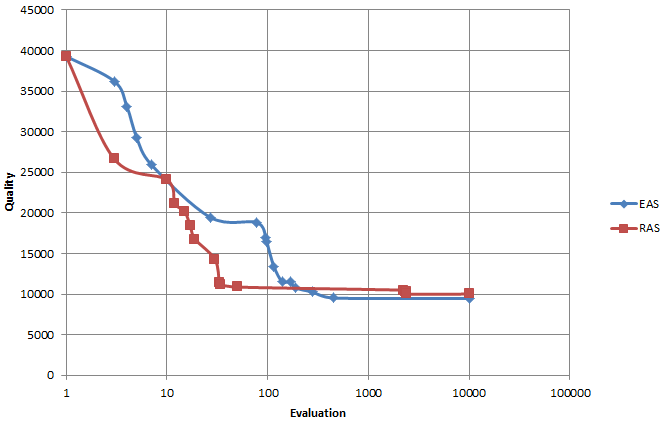
\includegraphics[scale=0.56]{no-ls.PNG}
  \caption{Performance convergence for the "chr15b.dat" instance by EAS and RAS without Local Search.}
  \label{fig:convergence-no-ls}
\end{figure}

\begin{figure}[H]
  \centering
    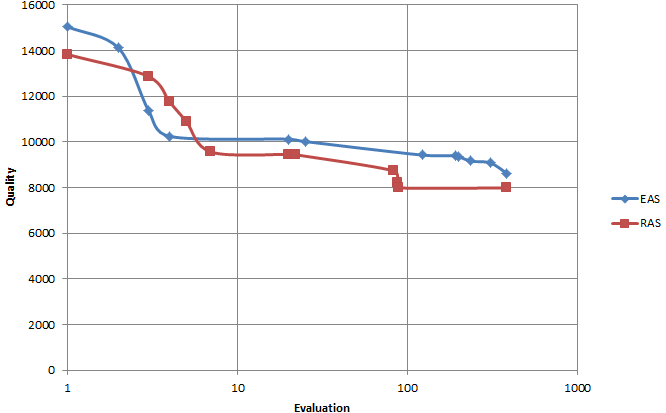
\includegraphics[scale=0.56]{ls-not-tuned.PNG}
  \caption{Performance convergence for the "chr15b.dat" instance by EAS and RAS with Local Search (not tuned).}
  \label{fig:convergence-ls-not-tuned}
\end{figure}

\begin{figure}[H]
  \centering
    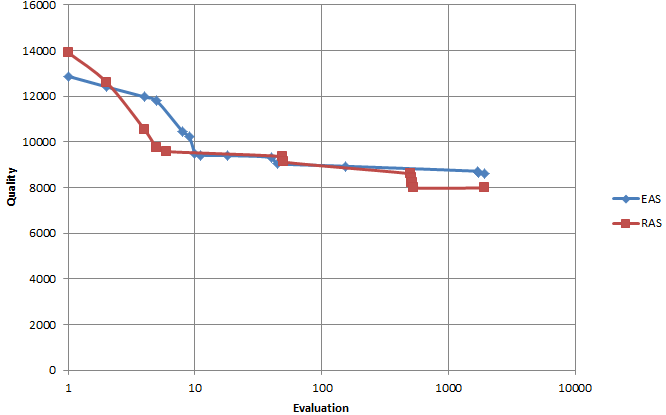
\includegraphics[scale=0.56]{ls-tuned.PNG}
  \caption{Performance convergence for the "chr15b.dat" instance by EAS and RAS with Local Search (tuned).}
  \label{fig:convergence-ls-tuned}
\end{figure}


\begin{table}[H]
\centering
\caption{Minimum solution qualities per each algorithm per each instance computed over 10 runs}
\label{tbl:experiment-min}
\begin{tabular}{|l|r|r|r|r|r|r|}
\hline
\textbf{Instance}   & \textbf{\thead{EAS \\(no LS)}} & \textbf{\thead{RAS \\(no LS)}} & \textbf{\thead{EAS (LS,\\ not tuned)}} & \textbf{\thead{RAS (LS, \\not tuned)}} & \textbf{\thead{EAS (LS,\\ tuned)}} & \textbf{\thead{RAS (LS,\\ tuned)}} \\ \hline
\textbf{bur26g.dat} & 9508105              & 9508105              & 9507884                      & 9507884                      & 9507884                  & 9507884                  \\ \hline
\textbf{chr15b.dat} & 8640                 & 8640                 & 7990                         & 7990                         & 7990                     & 7990                     \\ \hline
\textbf{esc16d.dat} & 16                   & 16                   & 16                           & 16                           & 16                       & 16                       \\ \hline
\textbf{had14.dat}  & 2724                 & 2724                 & 2724                         & 2724                         & 2724                     & 2724                     \\ \hline
\textbf{had20.dat}  & 6922                 & 6922                 & 6922                         & 6922                         & 6922                     & 6922                     \\ \hline
\textbf{nug28.dat}  & 5252                 & 5280                 & 5166                         & 5166                         & 5170                     & 5166                     \\ \hline
\textbf{scr12.dat}  & 31410                & 31410                & 31410                        & 31410                        & 31410                    & 31410                    \\ \hline
\textbf{tai17a.dat} & 504408               & 501058               & 493662                       & 491812                       & 493662                   & 493662                   \\ \hline
\textbf{tai35a.dat} & 2560610              & 2603248              & 2511090                      & 2513606                      & 2475022                  & 2470994                  \\ \hline
\textbf{wil50.dat}  & 49520                & 50058                & 48990                        & 48892                        & 48896                    & 48874                    \\ \hline
\end{tabular}
\end{table}

\begin{table}[H]
\centering
\caption{Maximum solution qualities per each algorithm per each instance computed over 10 runs}
\label{tbl:experiment-max}
\begin{tabular}{|l|r|r|r|r|r|r|}
\hline
\textbf{Instance}   & \textbf{\thead{EAS \\(no LS)}} & \textbf{\thead{RAS \\(no LS)}} & \textbf{\thead{EAS (LS,\\ not tuned)}} & \textbf{\thead{RAS (LS, \\not tuned)}} & \textbf{\thead{EAS (LS,\\ tuned)}} & \textbf{\thead{RAS (LS,\\ tuned)}} \\ \hline
\textbf{bur26g.dat} & 9549292              & 9586656              & 9508853                      & 9507884                      & 9508853                  & 9507884                  \\ \hline
\textbf{chr15b.dat} & 11978                & 11494                & 9290                         & 8626                         & 9290                     & 9290                     \\ \hline
\textbf{esc16d.dat} & 16                   & 16                   & 16                           & 16                           & 16                       & 16                       \\ \hline
\textbf{had14.dat}  & 2744                 & 2744                 & 2724                         & 2724                         & 2724                     & 2724                     \\ \hline
\textbf{had20.dat}  & 6964                 & 6972                 & 6948                         & 6922                         & 6922                     & 6948                     \\ \hline
\textbf{nug28.dat}  & 5442                 & 5358                 & 5252                         & 5228                         & 5272                     & 5254                     \\ \hline
\textbf{scr12.dat}  & 32996                & 32958                & 31410                        & 31410                        & 31410                    & 31410                    \\ \hline
\textbf{tai17a.dat} & 514492               & 516242               & 499670                       & 500790                       & 501326                   & 502304                   \\ \hline
\textbf{tai35a.dat} & 2660234              & 2680092              & 2541096                      & 2544234                      & 2504592                  & 2530968                  \\ \hline
\textbf{wil50.dat}  & 50354                & 51168                & 49152                        & 49056                        & 49028                    & 48996                    \\ \hline
\end{tabular}
\end{table}

\begin{table}[H]
\centering
\caption{Average solution qualities per each algorithm per each instance computed over 10 runs}
\label{tbl:experiment-average}
\begin{tabular}{|l|r|r|r|r|r|r|}
\hline
\textbf{Instance}   & \textbf{\thead{EAS \\(no LS)}} & \textbf{\thead{RAS \\(no LS)}} & \textbf{\thead{EAS (LS,\\ not tuned)}} & \textbf{\thead{RAS (LS, \\not tuned)}} & \textbf{\thead{EAS (LS,\\ tuned)}} & \textbf{\thead{RAS (LS,\\ tuned)}} \\ \hline
\textbf{bur26g.dat} & 9517432              & 9527396              & 9507980                      & 9507884                      & 9508174                  & 9507884                  \\ \hline
\textbf{chr15b.dat} & 10227                & 10093                & 8532                         & 8371                         & 8854                     & 8512                     \\ \hline
\textbf{esc16d.dat} & 16                   & 16                   & 16                           & 16                           & 16                       & 16                       \\ \hline
\textbf{had14.dat}  & 2730                 & 2734                 & 2724                         & 2724                         & 2724                     & 2724                     \\ \hline
\textbf{had20.dat}  & 6931                 & 6942                 & 6927                         & 6922                         & 6922                     & 6929                     \\ \hline
\textbf{nug28.dat}  & 5312                 & 5318                 & 5201                         & 5199                         & 5215                     & 5207                     \\ \hline
\textbf{scr12.dat}  & 32202                & 32123                & 31410                        & 31410                        & 31410                    & 31410                    \\ \hline
\textbf{tai17a.dat} & 510175               & 509739               & 495976                       & 496344                       & 498228                   & 497675                   \\ \hline
\textbf{tai35a.dat} & 2614268              & 2642542              & 2529051                      & 2532861                      & 2484877                  & 2488667                  \\ \hline
\textbf{wil50.dat}  & 49967                & 50503                & 49067                        & 48939                        & 48952                    & 48924                    \\ \hline
\end{tabular}
\end{table}


\begin{table}[H]
\centering
\caption{Standard deviations of solution qualities per each algorithm per each instance computed over 10 runs}
\label{tbl:experiment-deviation}
\begin{tabular}{|l|r|r|r|r|r|r|}
\hline
\textbf{Instance}   & \textbf{\thead{EAS \\(no LS)}} & \textbf{\thead{RAS \\(no LS)}} & \textbf{\thead{EAS (LS,\\ not tuned)}} & \textbf{\thead{RAS (LS, \\not tuned)}} & \textbf{\thead{EAS (LS,\\ tuned)}} & \textbf{\thead{RAS (LS,\\ tuned)}} \\ \hline
\textbf{bur26g.dat} & 16737.45             & 28934.45             & 306.43                       & 0                            & 468.07                   & 0                        \\ \hline
\textbf{chr15b.dat} & 1122.67              & 996.02               & 430.1                        & 328.43                       & 378.98                   & 495.72                   \\ \hline
\textbf{esc16d.dat} & 0                    & 0                    & 0                            & 0                            & 0                        & 0                        \\ \hline
\textbf{had14.dat}  & 9.66                 & 10.54                & 0                            & 0                            & 0                        & 0                        \\ \hline
\textbf{had20.dat}  & 14.34                & 18.4                 & 10.96                        & 0                            & 0                        & 12.59                    \\ \hline
\textbf{nug28.dat}  & 62.71                & 27.65                & 27.44                        & 18.36                        & 29.89                    & 28                       \\ \hline
\textbf{scr12.dat}  & 600.72               & 582.08               & 0                            & 0                            & 0                        & 0                        \\ \hline
\textbf{tai17a.dat} & 3286.57              & 4681.04              & 2334.31                      & 2780.92                      & 2286.86                  & 2986.83                  \\ \hline
\textbf{tai35a.dat} & 30049.49             & 24688.77             & 9590.59                      & 9326.62                      & 10462.45                 & 20092.04                 \\ \hline
\textbf{wil50.dat}  & 259.73               & 323.45               & 53.97                        & 45.09                        & 44.47                    & 43.72                    \\ \hline
\end{tabular}
\end{table}


\bibliographystyle{plain}
\bibliography{ref}

\end{document}

